%!TEX root = ../paper.tex

\begin{figure}[!ht]
\centering
\noindent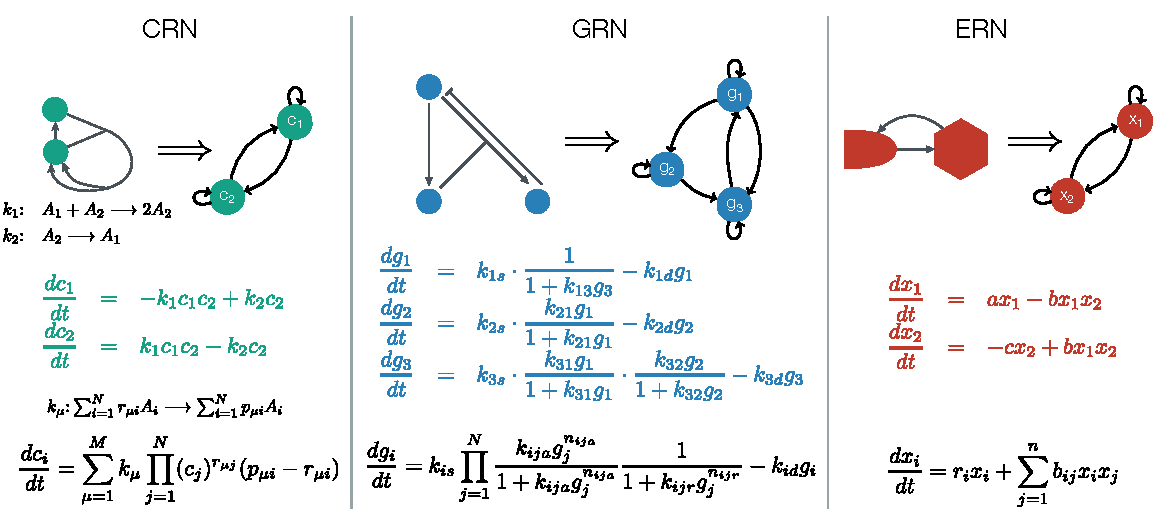
\includegraphics[width=0.9\columnwidth]{fig/biomodelexamples.pdf}
\caption{{\bf Dynamical models in systems biology.} (A) (B) (C)}
\label{fig:biomodelexamples}
\end{figure}

\pagebreak

\begin{figure}[!ht]
\centering
\noindent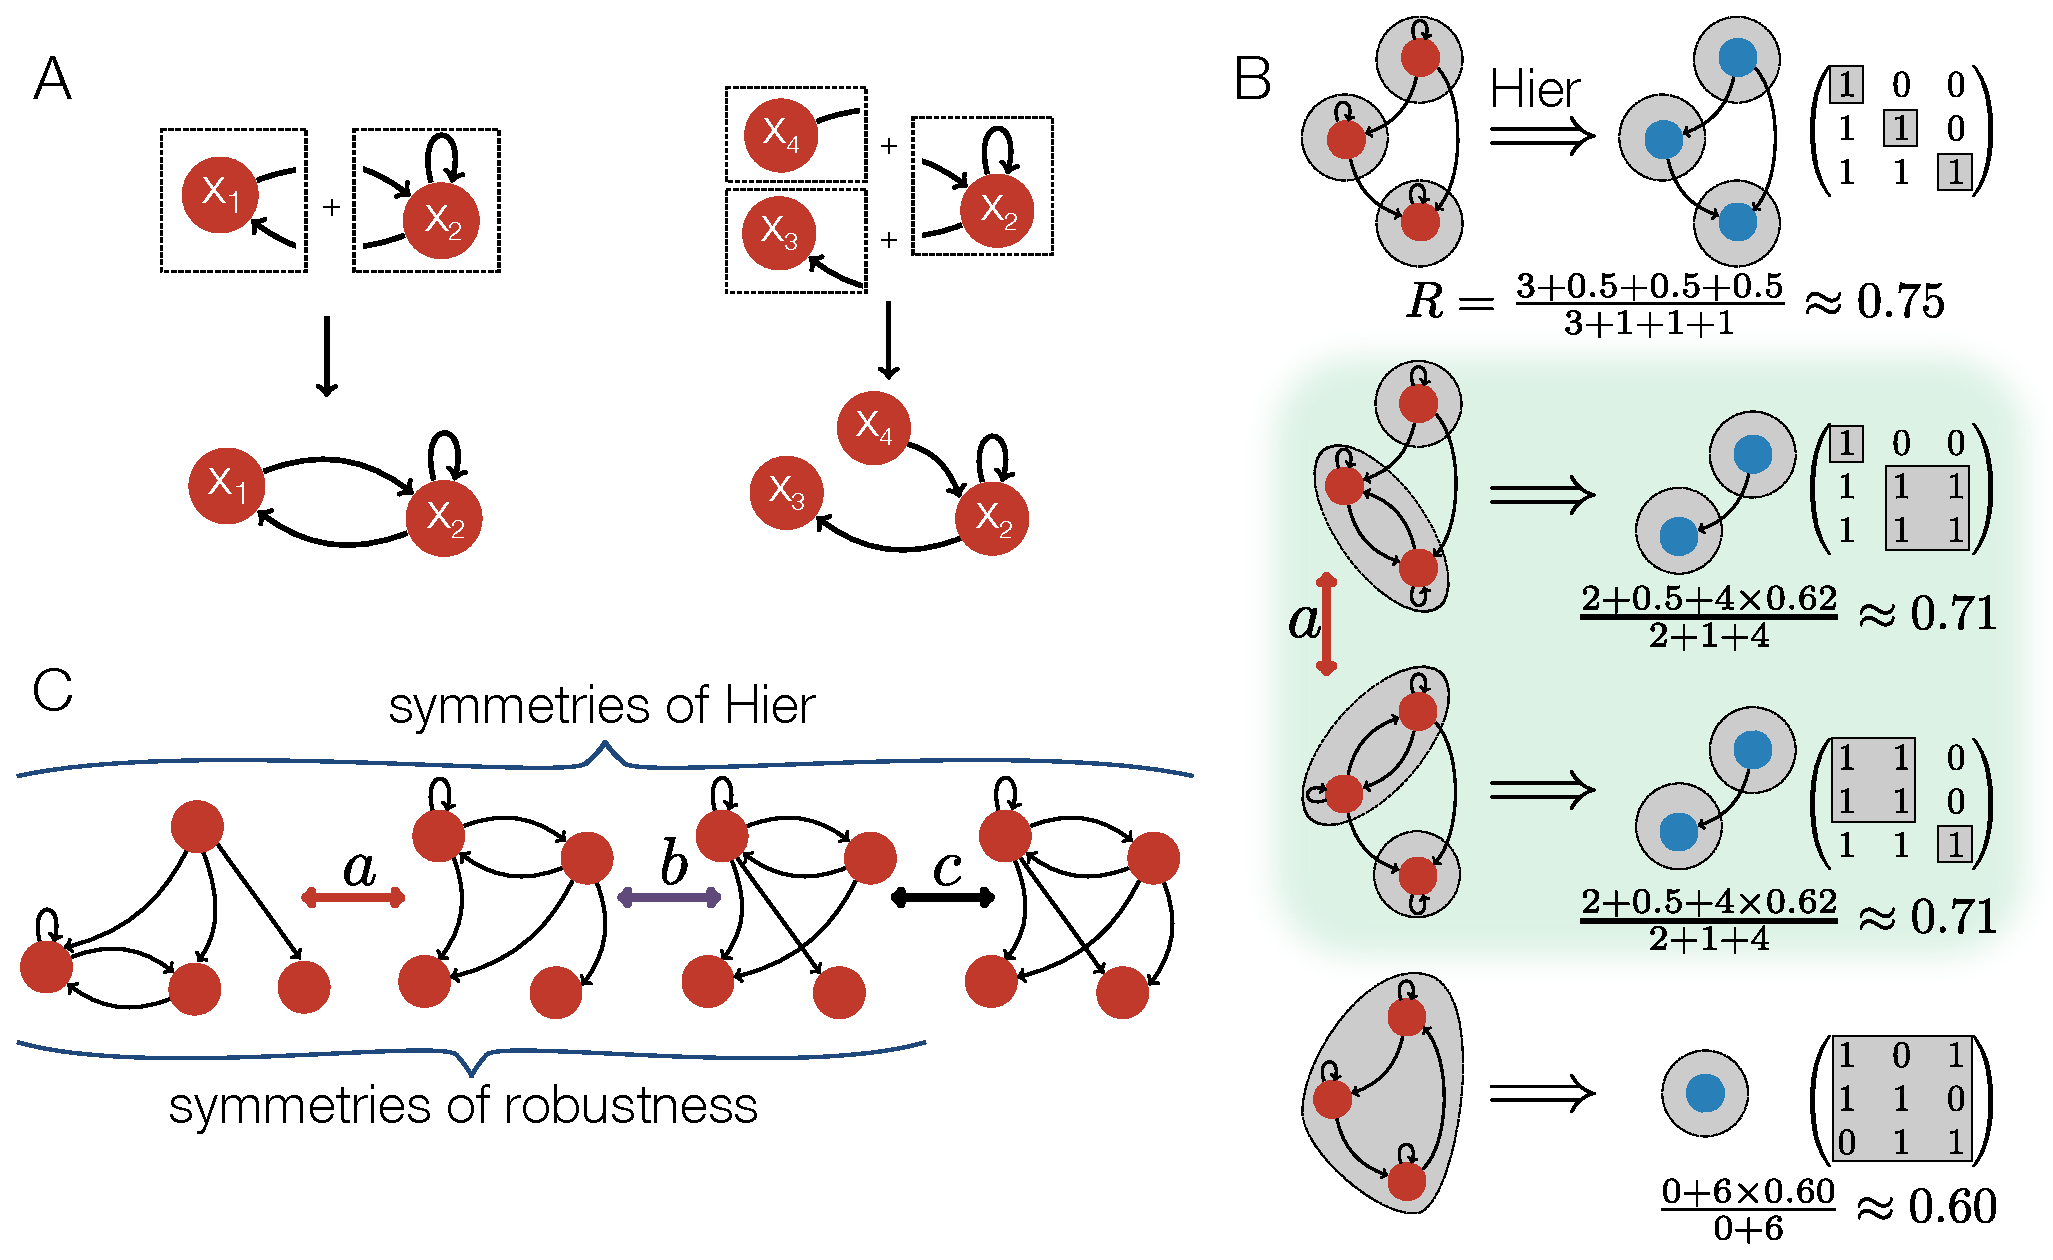
\includegraphics[width=0.9\columnwidth]{fig/modsccsym.pdf}
\caption{{\bf Open systems, strongly connected components and symmetries of robustness.} (A) Example of the combination of open system modules to construct closed systems. (B) strongly connected components highlighted in gray for each of the four graphs representing the interdependencies relevant to four different three component systems. The most hierarchical system in the top panel has the highest possible number of connected components, three, whereas the system in the bottom panel containing a single cycle and therefore posessing no hierarchy contains only one connected component. The two panels in the middle represent examples of hierarchical modular systems that posess both modularity and hierarchy. (C) Symmetries of the $\hier$ transformation between graphs and SCCs. The transformation a represents an interchange of SCCs, b moving a link between nodes in a component and c adding a link. All three transformations represent symmetries of the $\hier$ transformation from graphs to SCCs while only a and b are symmetries of robustness.}
\label{fig:modsccsym}
\end{figure}

\pagebreak


% \begin{figure}[!ht]
% \centering
% \noindent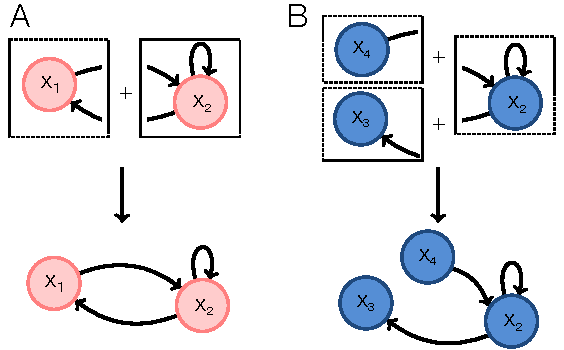
\includegraphics[width=0.4\columnwidth]{fig/examplesystemmodules.pdf}
% \caption{{\bf Example of the combination of open system modules to construct closed systems.} (A) Example of combining two open modules to construct a closed system of two components (B) Analogous example for combining three open modules to construct a closed system with three components}
% \label{fig:examplesystemmodules}
% \end{figure}

% \pagebreak

% \begin{figure}[!ht]
% \centering
% \noindent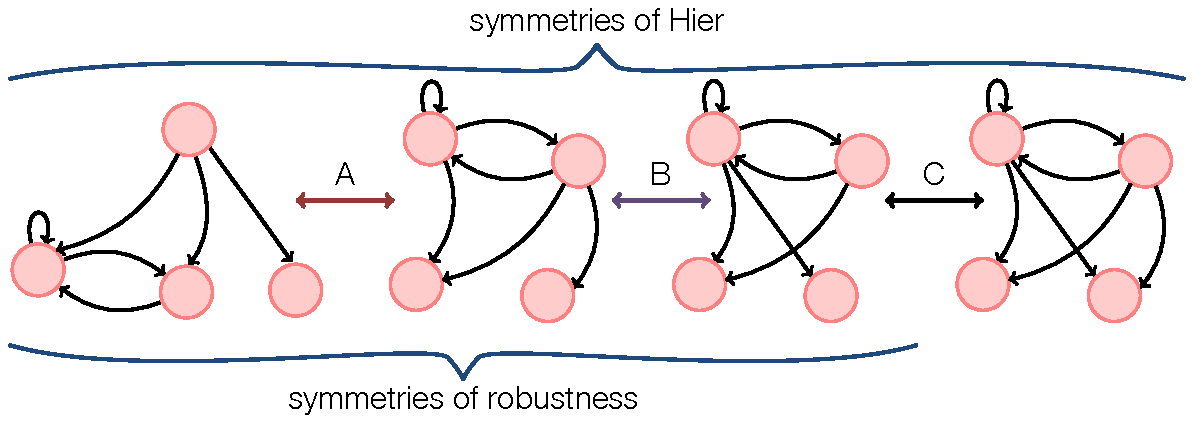
\includegraphics[width=0.7\columnwidth]{fig/hiertransformations.pdf}
% \caption{{\bf Symmetries of the $\hier$ transformation between graphs and SCCs.} The transformation A represents an interchange of SCCs, B moving a link between nodes in a component and C adding a link. All three transformations represent symmetries of the $\hier$ transformation from graphs to SCCs while only A and B are symmetries of robustness.}
% \label{fig:hiertransformations}
% \end{figure}

% \pagebreak

% \begin{figure}[!ht]
% \centering
% \noindent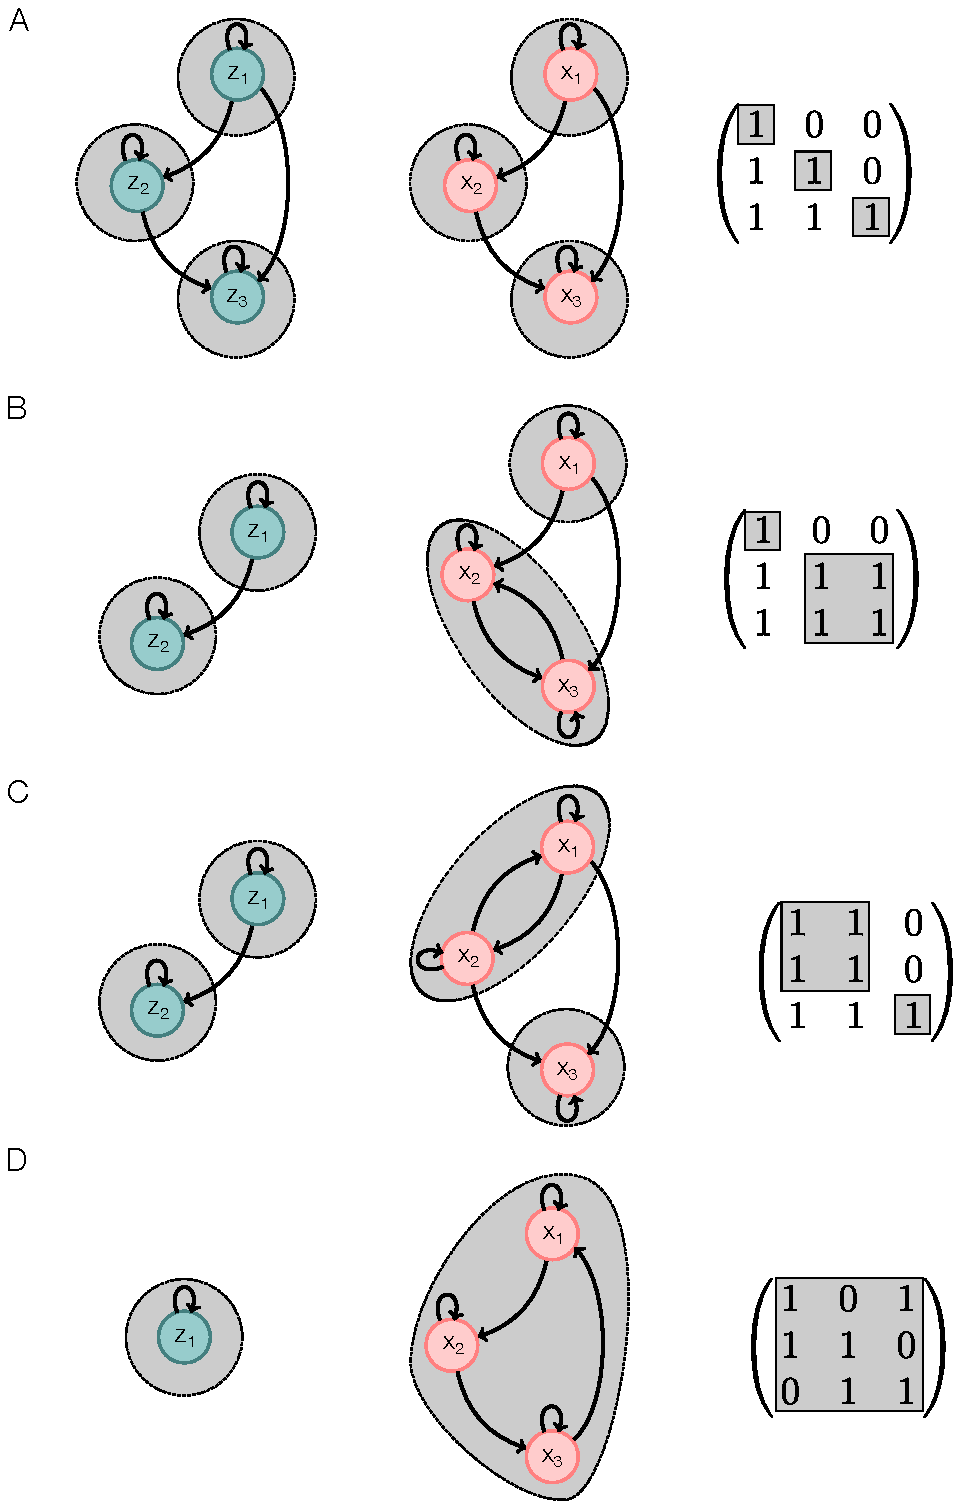
\includegraphics[width=0.4\columnwidth]{fig/scc2.pdf}
% \caption{{\bf Example of strongly connected components.} (A) - (D) show strongly connected components highlighted in gray for each of the four graphs representing the interdependencies relevant to four different three component systems. Note that the most hierarchical system in (A) has the highest possible number of connected components, three, whereas the system containing a single cycle and therefore posessing no hierarchy contains only one connected component. Systems (B) and (C) represent examples of hierarchical modular systems that posess both modularity and hierarchy.}
% \label{fig:scc}
% \end{figure}

% \pagebreak

\begin{figure}[!ht]
\centering
\noindent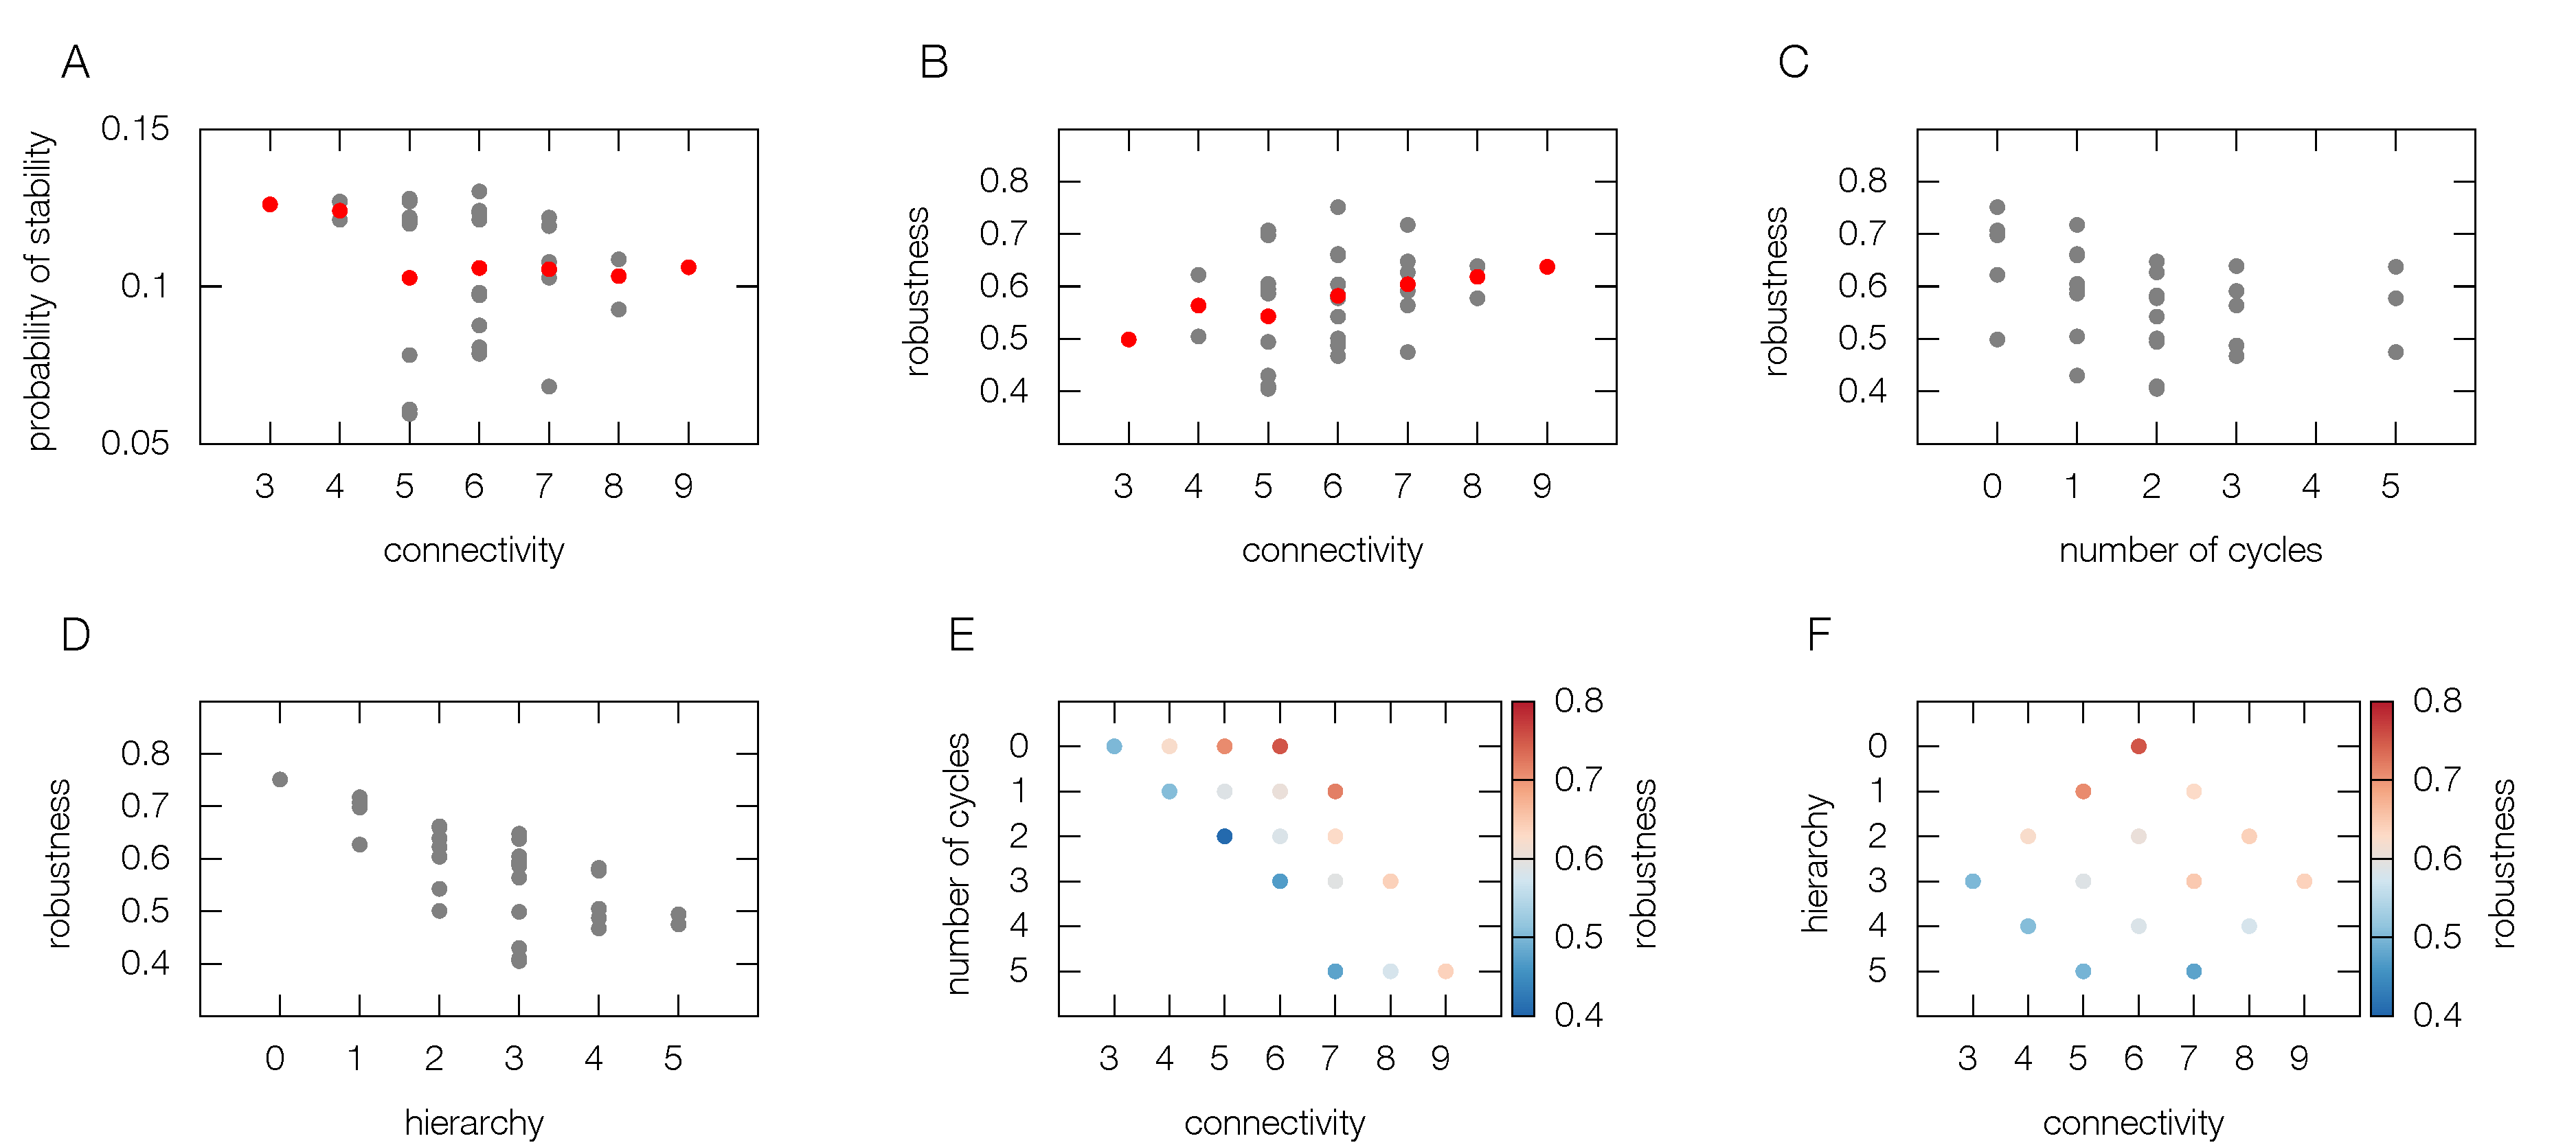
\includegraphics[width=1.0\columnwidth]{fig/combinedfigs.pdf}
\caption{{\bf Characterization of stability and robustness according to properties of system structure} (A) Stability versus connectivity, (B) robustness versus connectivity, (C) robustness versus number of cycles, (D) robustness versus hierarchy for three component systems.
}1,500 words long
\label{fig:combined}
\end{figure}

\pagebreak

\begin{figure}[!ht]
\centering
\noindent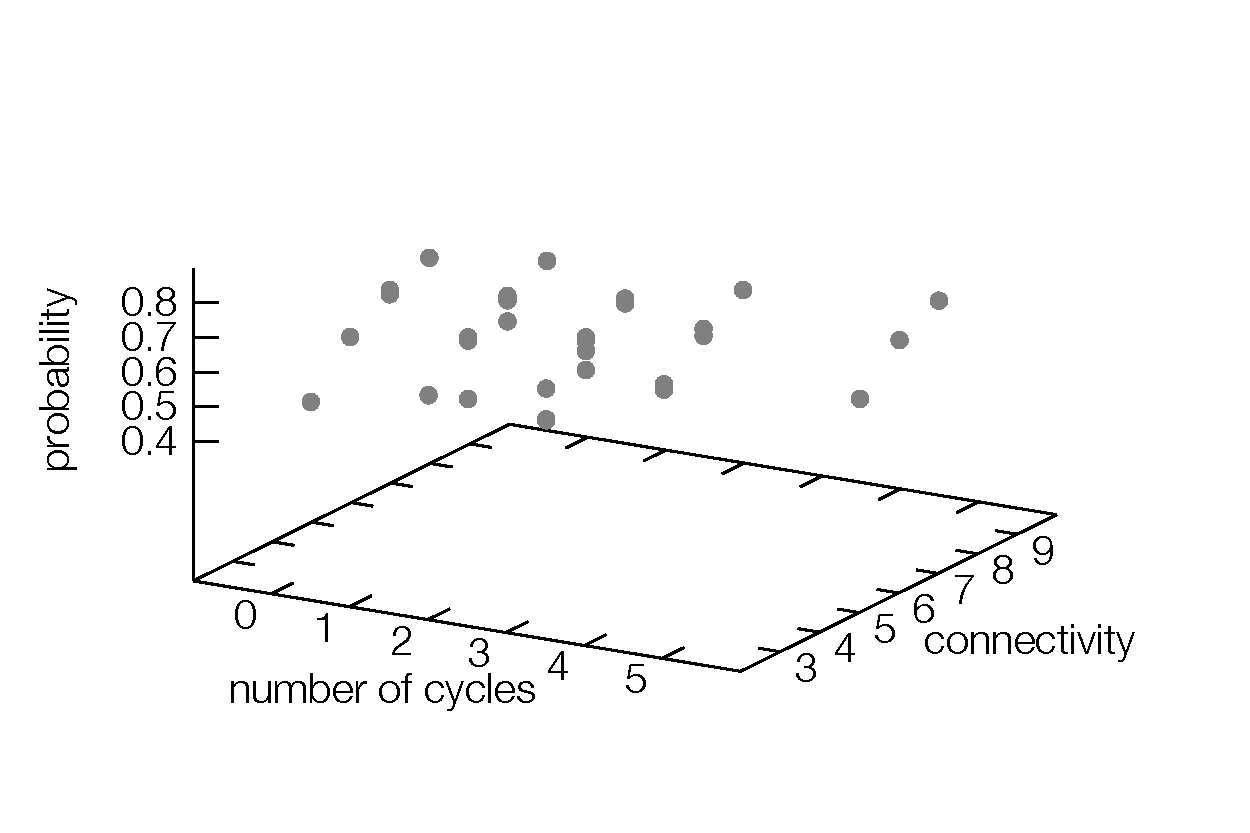
\includegraphics[width=0.8\columnwidth]{fig/connectcycle3D3x3.pdf}
\caption{{\bf Robustness versus number of cycles and connectivity for three component systems.} Each point represents the average robustness of all graphs having a given number of cycles and connectivity.}
\label{fig:connectcycle3D3x3}
\end{figure}

\pagebreak

\begin{figure}[!ht]
\centering
\noindent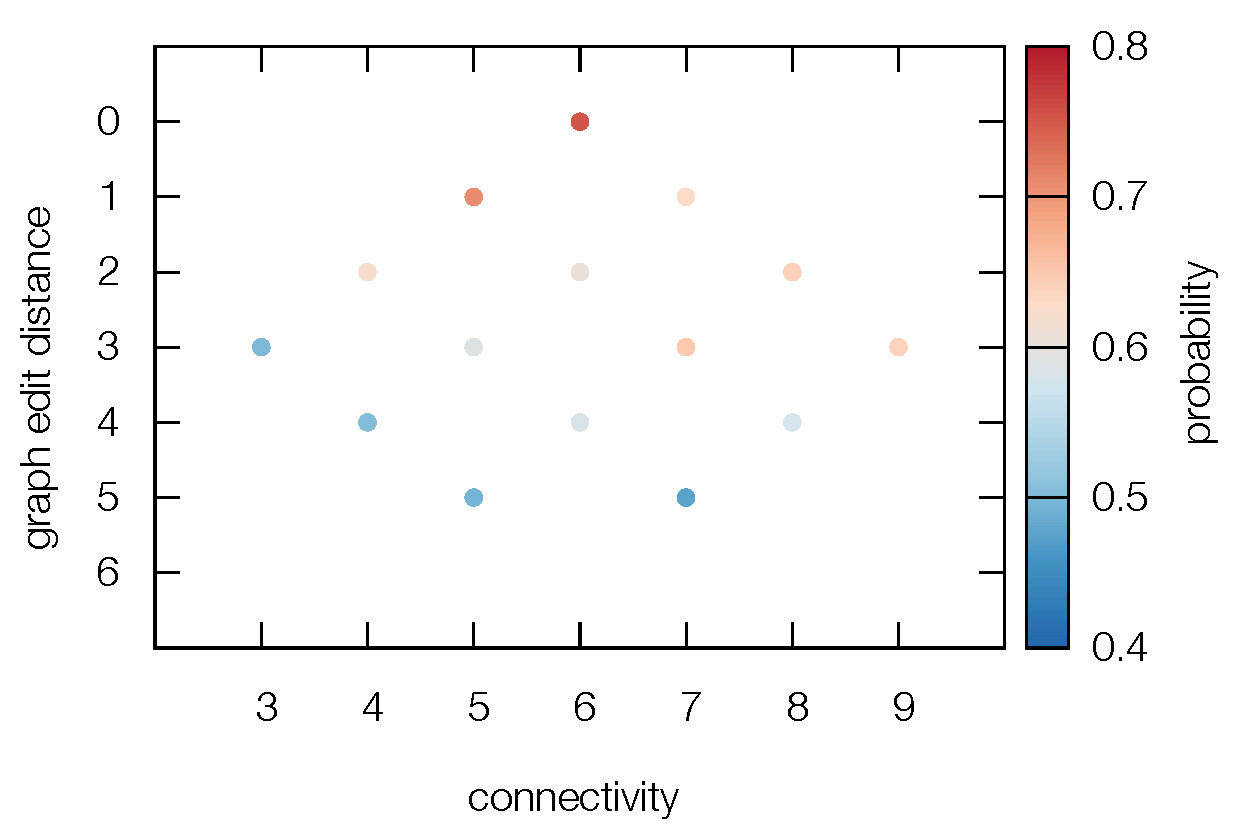
\includegraphics[width=0.8\columnwidth]{fig/connectdist3D3x3.pdf}
\caption{{\bf Robustness versus hierarchy and connectivity for three component systems.} Each point represents the average robustness of all graphs having a given hierarchy and connectivity.}
\label{fig:connectdist3D3x3}
\end{figure}

